\section{Methodology}

The present report uses \textit{EPOCH}\cite{EPOCH}, which is a fully relativistic, 3D, parallelized implementation of the particle-in-cell algorithm.

\subsection{PIC Approach}
% In plasma physics, the PIC method is a numerical approach that simulates a collection of particles that interact via external and self-induced electromagnetic fields. A spatial grid is used to describe the field while the particles move in the continuous space. The field and the particle motion are solved concurrently. In this case the simulation requires less amount of work, since each particle only interacts with the grid points of the cell where it is located.\cite{suciu}
The particle-in-cell (PIC) method is a numerical technique used in plasma physics to simulate the behavior of a group of particles interacting through both external and self-induced electromagnetic fields. The simulation is carried out on a spatial grid that describes the fields, while the particles move continuously through space. The motion of both the particles and the fields are solved simultaneously. Since each particle interacts only with the grid points of the cell it is located in, the simulation requires less computational effort. \cite{suciu}

In PIC, the plasma is represented by collection of particles, macro particle, with same charge to mass ratio. The system is discretised parallel to the boundaries forming a grid (mesh). The particles are free to move anywhere inside the system boundaries, however, the continuous electromagnetic field is replaced by discrete values assigned only to the mesh points.

The arrangement of the fields is called the Yee cell. Since the charge density is defined on the corners, the central difference places the electric fields at the edges. Meanwhile, the magnetic fields are located on the face. After the initial condition is given, PIC start by calculating the charge density ($\rho$) at grid points from nearby charged particles. The charge of each particle is distributed among the grid points using a weighting algorithm. Usually, a bilinear interpolation is used where the charge on the grid is determined using the subarea of the opposite vertex.

\begin{minipage}{0.50\textwidth}\raggedright
    In the PIC method, after setting the initial conditions, the next step is to compute the charge density ($\rho$) at each grid point by gathering the contribution from nearby charged particles. The charge of each particle is distributed among the grid points using a weighting algorithm. Usually, a bilinear interpolation is used where the charge on the grid is determined using the subarea of the opposite vertex.
\end{minipage}
\begin{minipage}{0.45\textwidth}\raggedleft
    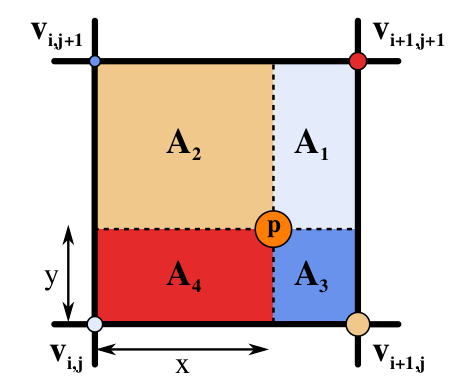
\includegraphics[height=5cm, width=7cm]{charge.png}
\end{minipage}

\begin{minipage}{0.55\textwidth}\raggedright
    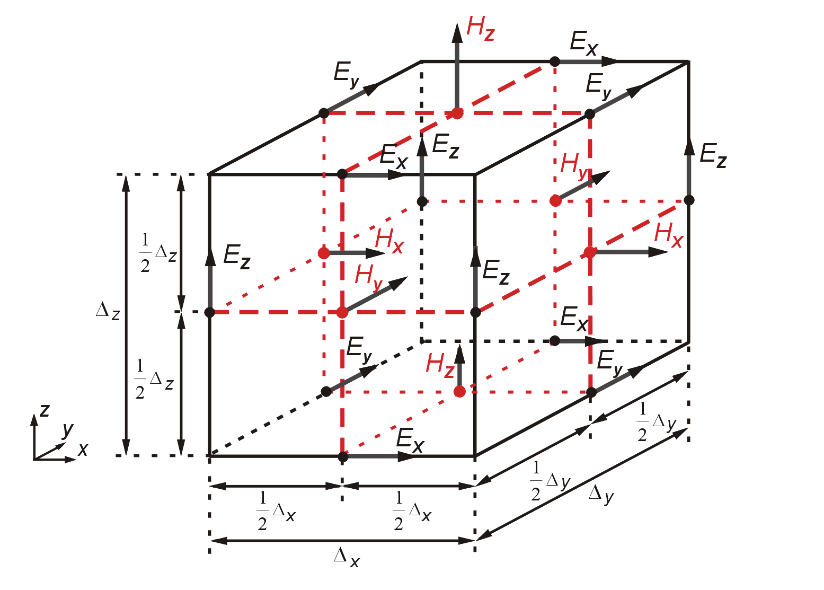
\includegraphics[height=7cm, width=9cm]{yee.png}
\end{minipage}
\begin{minipage}{0.40\textwidth}\raggedright
    The Yee cell is a staggered grid arrangement used in (PIC) simulations to determine the positions of electric and magnetic field nodes. In this scheme, the electric field components are located at the faces of the cubic cell, while the magnetic field components are located at the edges of the cell. This arrangement ensures accurate and stable time integration of the fields in PIC simulations, making it a widely used scheme in simulating electromagnetic phenomena in plasmas and other complex systems.
\end{minipage}

Update of $\mathbf{E}$ and $\mathbf{B}$ is done by Yee algorithm. The advancement of $\mathbf{E}$ from step $n$ to $n+1$ is done via central differencing using $\mathbf{B}$ at $n+1/2$. While, the advancement of $\mathbf{B}$ from step $n-1/2$ to $n+1/2$ is done via central differencing using $\mathbf{E}$ and the current density ($\textbf{J}$) at step $n$. Finally, the updated electric and magnetic fields are used to forward velocity for step $n-1/2$ to $n+1/2$ and velocity at step $n+1/2$ is used to forward position for step $n$ to $n+1$. The charge and hence the current density is updated using this newly updated position which in turn updates magnetic field and the cycle continues. The fact that the velocity ($\mathbf{B}$) at half step is used to forward position ($\mathbf{E}$) at full step and vice versa makes this update rule leap-frog method.

\begin{figure}[H]
    \centering
    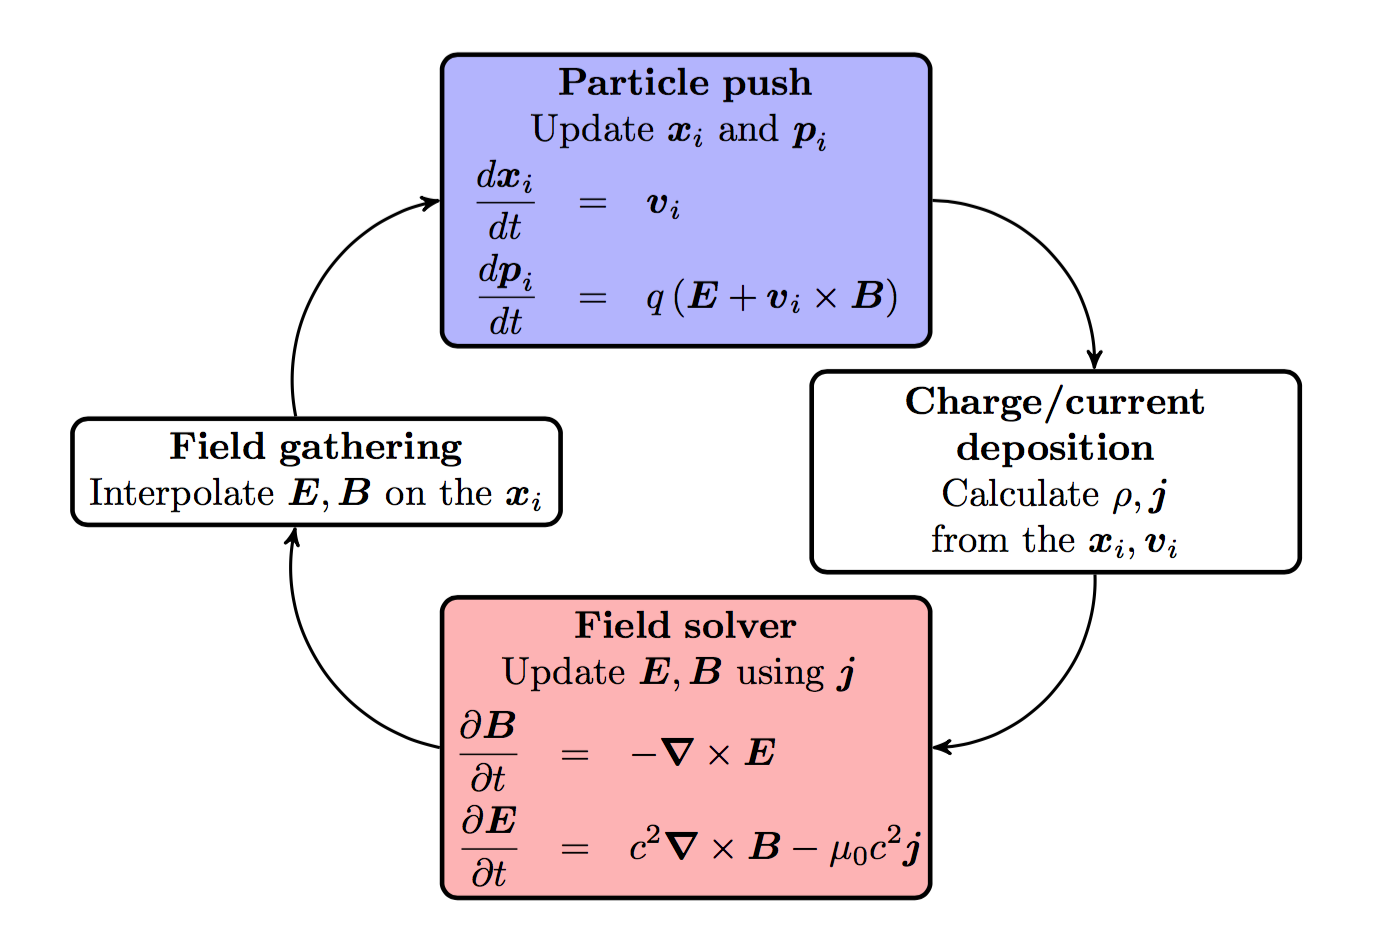
\includegraphics[width=0.9\textwidth]{pic_loop.png}
    \caption{The four steps of a PIC cycle.}
    \label{fig:pic-loop}
\end{figure}

The velocity is updated with Boris method. First, a half-step acceleration is performed in the electric field direction, followed by full rotation in magnetic field and finally, another half-step acceleration is performed in the electric field direction.

\subsection{Simulation Setup}
The present report includes two types of simulations: first, we use a normally incident laser pulse to study the effect of various laser and plasma parameters on generated HHG. Secondly, we have performed some simulations to study the oblique incidence and different polarization.

\subsubsection{For Normal Incident}
Before, going to the main study, we have performed some preliminary simulations to study how relativistic and non-relativistic laser interact with overdense and underdense plasma. After this, the effect of various laser and plasma parameters on generated HHG are studied. The simulation setup for both simulations is given below.

\subsubsubsection{Simulation Setup for Preliminary Study}\label{sec:preliminary}
The simulation box extends for $20 \lambda _l$ (from $-10 \lambda _l$ to $10 \lambda _l$), where $\lambda_l$ is the laser wavelength and has total 1000 cells, i.e., 50 cells per wavelength. The plasma is placed at $x=0$ and with a thickess of $\lambda_l$. Number of particles per cell are 100.  The plasma density $n_p$ is defined in terms of the critical density $n_c$ and is varied from 0.1 to 10. The vector potential $a_0$ of the laser pulse is also varied as 0.1, 1.0 and 10 for each set of plasma density. The laser envelope is used for this simulation is sine-squared, see equation \ref{eq:sin-sq-env}. Where T is the pulse duration here taken as $T=10\tau$ with $\tau = 2\pi/\omega_l$ is the time of one laser cycle. The simulation is performed for $t=20\tau$.

\subsubsubsection{Simulation Setup for HHG Study}\label{sec:normal_hhg}
The simulation box extends for $40 \lambda _l$ (from $-20 \lambda _l$ to $20 \lambda _l$), where $\lambda_l$ is the laser wavelength taken as $1\mu m$ and has a total of 16000 cells, i.e., 400 cells per wavelength. The plasma is placed at $x=0$ and with a thickness of $\lambda_l$. The number of particles per cell is 100. The pulse duration is $T = 20 \tau$ and the simulation is run till $T_{end} = 40 \tau$. Here $\tau$ is the time period of the laser pulse. We have studied effects of different laser envelopes that are given below:
% \begin{equation}
%     \label{eq:sg}
%     P = P_0 \exp\left( -2 \left(\frac{x - \mu}{\sigma}\right)^p\right)
% \end{equation}
% where $P_0$ is the normalization constant, $\mu$ is the mean, $\sigma$ is the standard deviation and $p$ is the power of the SG.

\noindent
1. Sine Sqaured
\begin{equation}
    \label{eq:sin-sq-env}
    P(t)=
    \begin{cases}
         & \sin^2(\pi t/T) \text{ for } 0 \leq t \le T \\
         & 0         \;      \text{ otherwise }
    \end{cases}
\end{equation}
2. Gaussian
\begin{equation}
    \label{eq:gaussian-env}
    P(t)=
    \begin{cases}
         & e^{\frac{-(t-T/2)^2}{2(0.2T)^2}} \text{ for } 0 \leq t \le T \\
         & 0         \;      \text{ otherwise }
    \end{cases}
\end{equation}
3. Triangular
\begin{equation}
    \label{eq:triangle-env}
    P(t)= 2\times
    \begin{cases}
         & t/T \text{ for } 0 \leq t \le T/2    \\
         & 1-t/T \text{ for } T/2 \leq t \le T  \\
         & 0         \;      \text{ otherwise }
    \end{cases}
\end{equation}
4. Super-Gaussian
\begin{equation}
    \label{eq:sg-env}
    P(t)=
    \begin{cases}
         & e^{\frac{-(t-T/2)^p}{2(0.2T)^p}} \text{ for } 0 \leq t \le T \\
         & 0         \;      \text{ otherwise }
    \end{cases}
\end{equation}

Here $T$ is the pulse duration and $t$ is the time. The pulse duration is taken as $T = 20 \tau$. $p$ is the power of the SG envelope. We also studied the effect of power of SG envelope on generated HHG.

\subsubsection{For Oblique Incident}
To report uses only a 1D simulation for oblique incidence. This is accommodated by following Bourdier transformation\cite{2d-transformation}, where simulations are performed in a frame which is moving in such a way that the light is normally incident. (See figure \ref{fig:frames})

\begin{figure}[H]
    \centering
    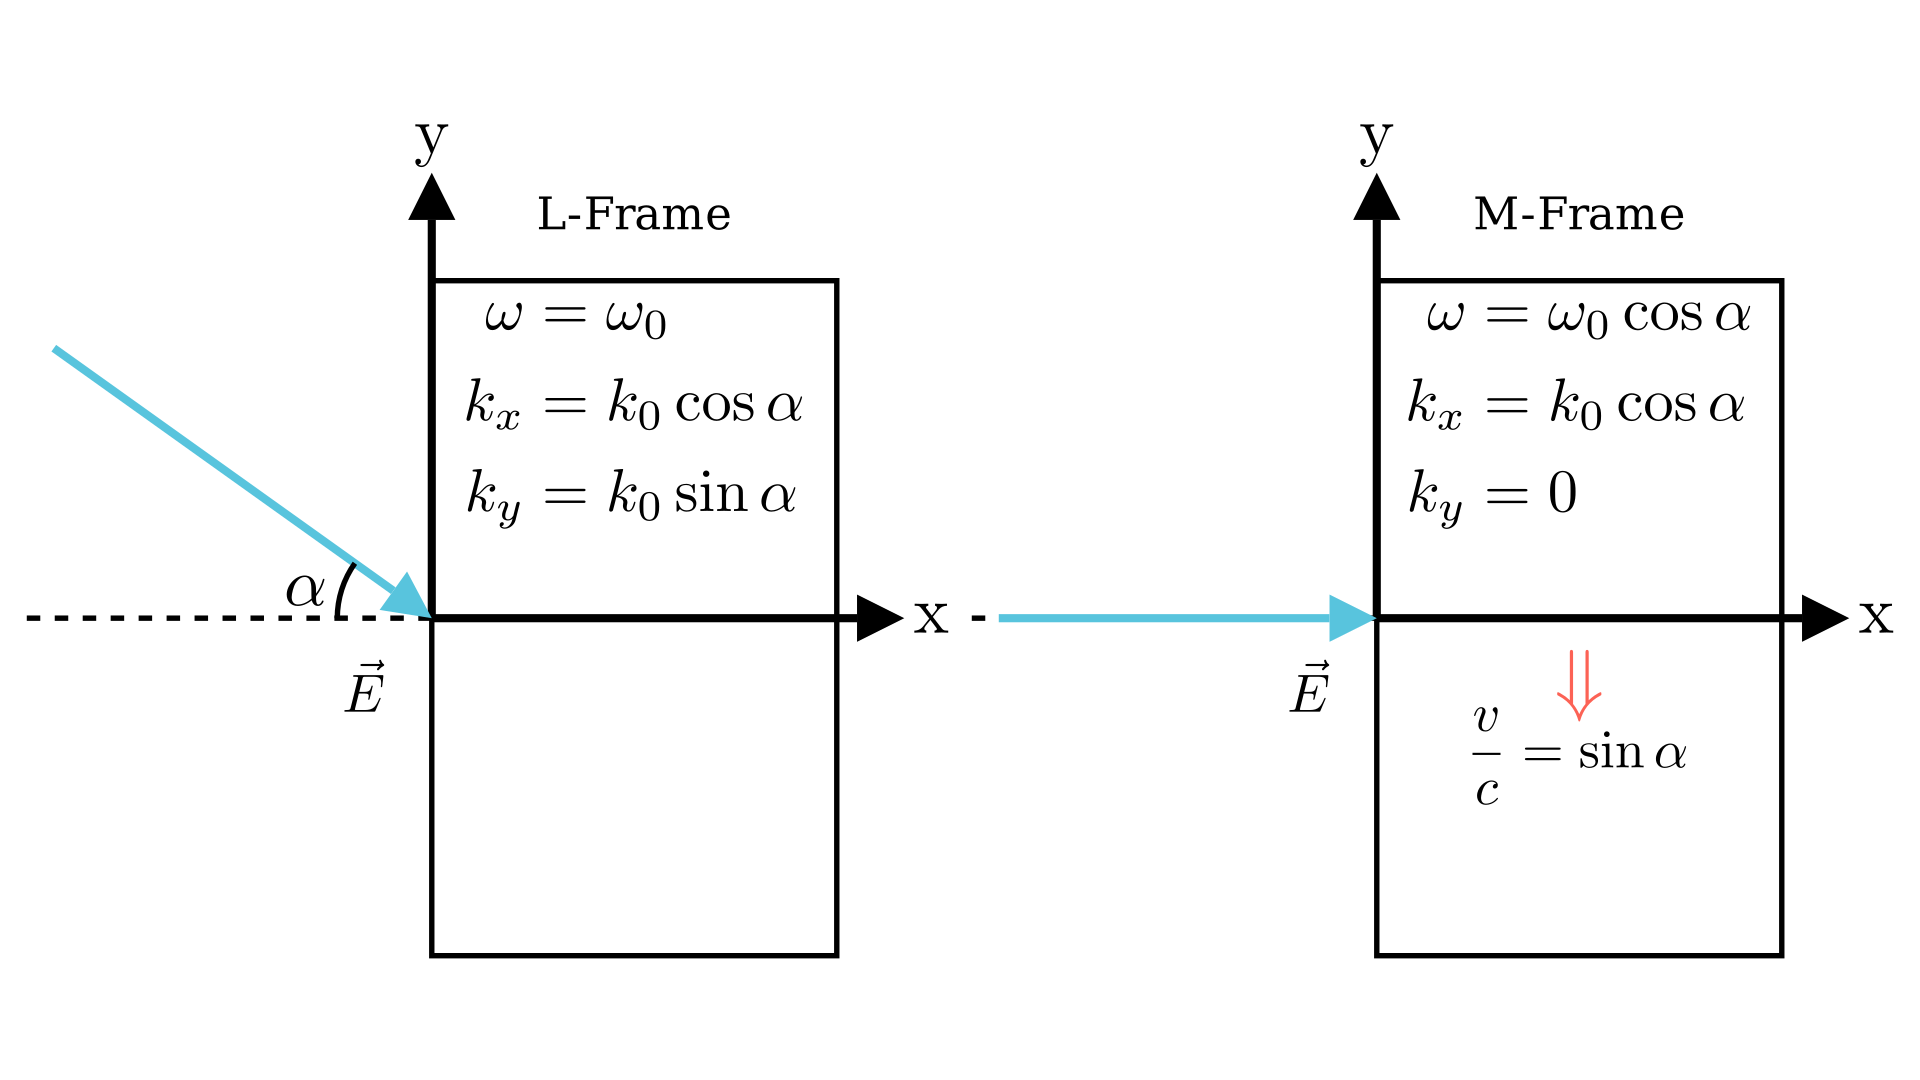
\includegraphics[width=1\textwidth]{frames.png}
    \centering
    \caption{L is the lab frame and M is the moving frame. Simulations are done in the M-frame and then they are transformed back to the L-Frame}
    \label{fig:frames}
\end{figure}

\subsubsubsection{Bourdier transformation}

For this, we make a Lorentz transformation from the laboratory frame L to frame M, moving with a velocity of $\mathbf{v_M} = c\sin\alpha \hat{y}$. As the frame is moving in $y$ direction and the speed is $c\sin\alpha$, the incident pulse is normal to the surface in the M-frame as illustracted in Figure \ref{fig:frames}. This means that the plasma must be moving with a velocity of $-\mathbf{v_f}$. The frequency $\omega_0$ and the wave vector $\mathbf{k}_0$ changes so that the speed of light is the same. The transformations of these are in figure \ref{fig:frames}.

% \begin{figure}[h]
%     \begin{minipage}{0.4\textwidth}\raggedright
%         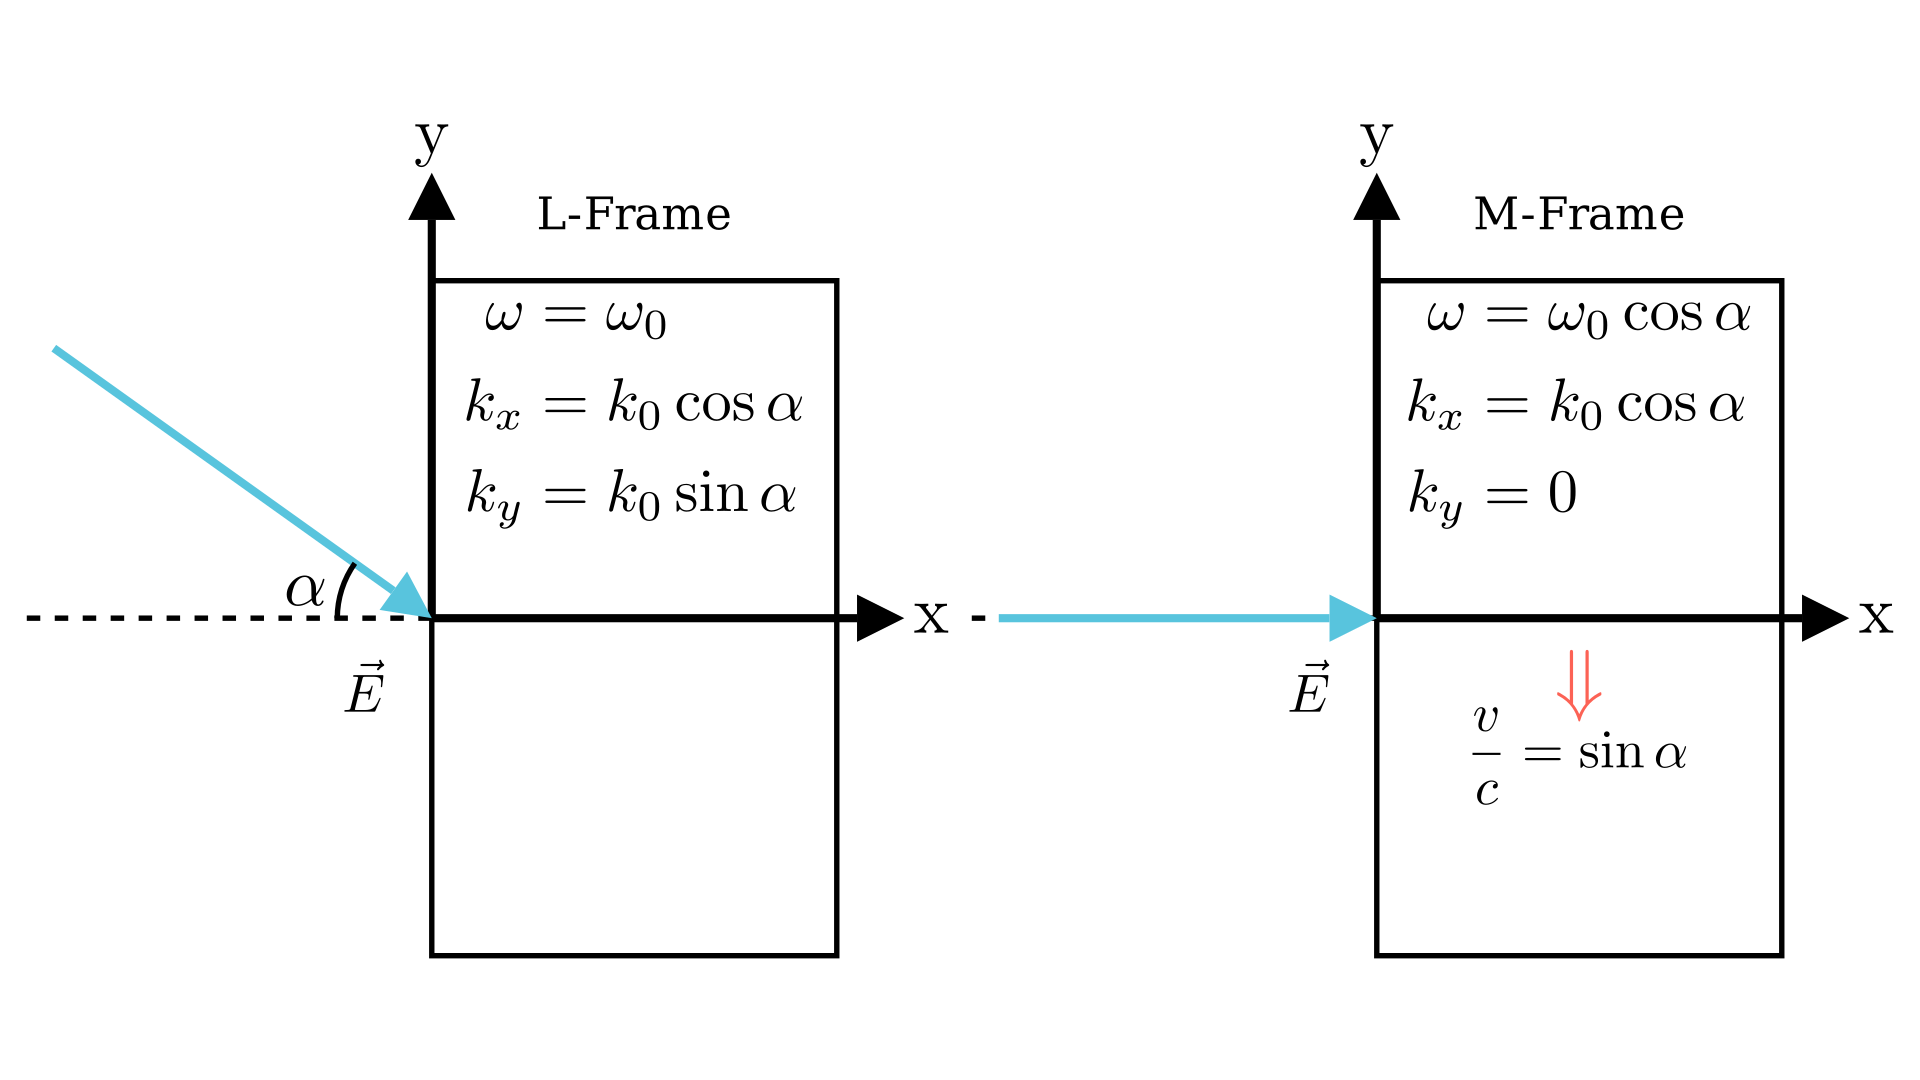
\includegraphics[width=1\textwidth]{frames.png}
%         \caption{L is the lab frame and M is the moving frame. Simulations are done in the M-frame and then they are transformed back to the L-Frame}
%         \label{fig:frames}
%     \end{minipage}
% \end{figure}
% \begin{table}[h]
%     \begin{minipage}{0.40\textwidth}
%         \centering
%         \caption{Transformation Equations}
%         \label{tab:transformation}
%         \vspace{0.3cm}
%         \begin{tabular}{|l|l|l|}
%             \hline
%             \textbf{Quantity}          & \textbf{L-Frame}                                 & \textbf{M-Frame}          \\ \hline
%             $\omega$                   & $\omega_0$                                       & $\omega_0 \cos\alpha$     \\ \hline
%             $\lambda$                  & $\lambda_0$                                      & $\lambda_0/\cos\alpha$    \\ \hline
%             $n$                        & $n_0$                                            & $n_0/\cos\alpha$          \\ \hline
%             $\mathbf{E}$ (p-polarized) & $E_0 (-\sin\alpha \hat{x} + \cos\alpha \hat{y})$ & $E_0 \cos\alpha \hat{y}$  \\ \hline
%             $\mathbf{E}$ (s-polarized) & $E_0 \hat{z}$                                    & $E_0 \cos\alpha \hat{z}$  \\ \hline
%             $\mathbf{B}$ (p-polarized) & $E_0 \hat{z}$                                    & $E_0 \cos\alpha \hat{z}$  \\ \hline
%             $\mathbf{B}$ (s-polarized) & $E_0 (\sin\alpha \hat{x} - \cos\alpha \hat{y})$  & $-E_0 \cos\alpha \hat{y}$ \\ \hline
%         \end{tabular}
%     \end{minipage}
% \end{table}



% \begin{align}
%     \label{fig:omega-k}
%     \begin{split}
%         \omega_L     & = \omega_0                                      \\
%         \omega_M     & = \omega_0\cos\alpha                            \\
%         \mathbf{k}_L & = k_0\cos\alpha \hat{x} + k_0\sin\alpha \hat{y} \\
%         \mathbf{k}_M & = k_0\cos\alpha \hat{x}
%     \end{split}
% \end{align}

The electric and magnetic field also changes. For p-polarization, the transformation equations are:

\begin{align}
    \label{eq:field-p}
    \begin{split}
        \mathbf{E}_L  & = E_0(-\sin\alpha \hat{x} + \cos\alpha \hat{y}) \\
        \mathbf{E}_M  & = E_0\cos\alpha \hat{y}                         \\
        c\mathbf{B}_L & = E_0\hat{z}                                    \\
        c\mathbf{B}_M & = E_0\cos\alpha \hat{z}
    \end{split}
\end{align}

While for s-polarization:

\begin{align}
    \label{eq:field-s}
    \begin{split}
        \mathbf{E}_L & = E_0\hat{z}                                    \\
        \mathbf{E}_M & = E_0\cos\alpha \hat{z}                        \\
        c\mathbf{B}_L & = E_0(\sin\alpha \hat{x} - \cos\alpha \hat{y}) \\
        c\mathbf{B}_M & = -E_0\cos\alpha \hat{y}
    \end{split}
\end{align}

Note that the amplitudes of the field are scaled down by a factor of $\cos\alpha$ and hence intensity also decreases. However, the normalized vector potential $a_0 = eE_0/m\omega_0c$ remains invariant. The density becomes $n_M = n_0/\cos\alpha$. A summary of these transformations is given in the table below:
\begin{table}[h]
    \centering
    \caption{Transformation Equations}
    \label{tab:transformation}
    \vspace{0.3cm}
    \begin{tabular}{|l|l|l|}
        \hline
        \textbf{Quantity}          & \textbf{L-Frame}                                 & \textbf{M-Frame}          \\ \hline
        $\omega$                   & $\omega_l$                                       & $\omega_l \cos\alpha$     \\ \hline
        $\lambda$                  & $\lambda_l$                                      & $\lambda_l/\cos\alpha$    \\ \hline
        $n$                        & $n_0$                                            & $n_0/\cos\alpha$          \\ \hline
        $\mathbf{E}$ (p-polarized) & $E_0 (-\sin\alpha \hat{x} + \cos\alpha \hat{y})$ & $E_0 \cos\alpha \hat{y}$  \\ \hline
        $\mathbf{E}$ (s-polarized) & $E_0 \hat{z}$                                    & $E_0 \cos\alpha \hat{z}$  \\ \hline
        $\mathbf{B}$ (p-polarized) & $E_0 \hat{z}$                                    & $E_0 \cos\alpha \hat{z}$  \\ \hline
        $\mathbf{B}$ (s-polarized) & $E_0 (\sin\alpha \hat{x} - \cos\alpha \hat{y})$  & $-E_0 \cos\alpha \hat{y}$ \\ \hline
    \end{tabular}
\end{table}
\subsubsubsection{Simulation Setup for Oblique Incident}\label{sec:oblique_hhg}
The simulation box extends for $40 \lambda _l$ (from $-20 \lambda _l$ to $20 \lambda _l$), where $\lambda_l$ is the laser wavelength taken as $1\mu m$ and has a total of 16000 cells, i.e., 400 cells per wavelength. The plasma is placed at $x=0$ and with a thickness of $\lambda_l$. The number of particles per cell is 100. The pulse duration is $T = 20 \tau$ and the simulation is run till $T_{end} = 40 \tau$
